
%%%%%%%%%%%%%%%%%%%%%%% file typeinst.tex %%%%%%%%%%%%%%%%%%%%%%%%%
%
% This is the LaTeX source for the instructions to authors using
% the LaTeX document class 'llncs.cls' for contributions to
% the Lecture Notes in Computer Sciences series.
% http://www.springer.com/lncs       Springer Heidelberg 2006/05/04
%
% It may be used as a template for your own input - copy it
% to a new file with a new name and use it as the basis
% for your article.
%
% NB: the document class 'llncs' has its own and detailed documentation, see
% ftp://ftp.springer.de/data/pubftp/pub/tex/latex/llncs/latex2e/llncsdoc.pdf
%
%%%%%%%%%%%%%%%%%%%%%%%%%%%%%%%%%%%%%%%%%%%%%%%%%%%%%%%%%%%%%%%%%%%


\documentclass[runningheads,a4paper]{llncs}

\usepackage{amssymb}
\setcounter{tocdepth}{3}
\usepackage{graphicx}

\usepackage{url}
\urldef{\mailsa}\path|{syshen,yingqin,|
\urldef{\mailsb}\path|jmzhang,|
\urldef{\mailsc}\path|skli}@nudt.edu.cn|
\newcommand{\keywords}[1]{\par\addvspace\baselineskip
\noindent\keywordname\enspace\ignorespaces#1}

\newtheorem{algorithm}{Algorithm}

\begin{document}

\mainmatter  % start of an individual contribution

% first the title is needed
%\title{Lecture Notes in Computer Science:\\Authors' Instructions
%for the Preparation\\of Camera-Ready
%Contributions\\to LNCS/LNAI/LNBI Proceedings}
\title{CompSyn : A Tool for Automatically Synthesizing Decoders}

% a short form should be given in case it is too long for the running head
%\titlerunning{Lecture Notes in Computer Science: Authors' Instructions}

% the name(s) of the author(s) follow(s) next
%
% NB: Chinese authors should write their first names(s) in front of
% their surnames. This ensures that the names appear correctly in
% the running heads and the author index.
%
\author{ShengYu Shen%
%\thanks{Project 61070132 supported by National Natural Science Foundation of China.}%
\and Ying Qin\and JianMin Zhang\and SiKun Li}
%
\authorrunning{ShengYu Shen\and Ying Qin\and JianMin Zhang\and SiKun Li}
% (feature abused for this document to repeat the title also on left hand pages)

% the affiliations are given next; don't give your e-mail address
% unless you accept that it will be published
\institute{School of Computer, National University of Defense Technology, China\\
\mailsa\mailsb\mailsc\\
\url{http://www.ssypub.org/}}

%
% NB: a more complex sample for affiliations and the mapping to the
% corresponding authors can be found in the file "llncs.dem"
% (search for the string "\mainmatter" where a contribution starts).
% "llncs.dem" accompanies the document class "llncs.cls".
%

\toctitle{Lecture Notes in Computer Science}
\tocauthor{Authors' Instructions}
\maketitle


\begin{abstract}
CompSyn is a tool that automatically synthesizes a decoder circuit from an encoder and a predefined assertion.
This tool has two usage modes: the synthesis mode and inferring mode.

\vspace{0.1cm}

When the correct assertion is known,
\textbf{the synthesis mode} is used to determine the existence of the decoder and generate it;
When the assertion is not known,
\textbf{the inferring mode} is used to infer this assertion and generate all possible decoders.
To help the user select the correct decoder,
this mode also infers each decoder's precondition formula,
which represents the set of assertions that can generate this decoder.

\vspace{0.1cm}

Experimental results show that
this tool can infer assertions and generate decoders for several complex encoders,
including PCI-E and Ethernet.
And the human effort in specifying assertion is significantly reduced.

\keywords{Complementary Synthesis, Inferring Assertion}
\end{abstract}


\section{Introduction}\label{sec_intro}
One of the most difficult jobs in designing communication chips
is to design and verify the complex complementary circuit pair $(E,E^{-1})$,
in which the encoder $E$ transforms information into a format suitable for transmission,
while its complementary circuit(or decoder) $E^{-1}$ recovers this information.

In order to facilitate this job,
we propose the complementary synthesis algorithm \cite{ShengYuShen:iccad09,ShengYuShen:tcad,ShengYuShen:tcad11,ShengYuShen:iccad11},
and develop the CompSyn tool to automatically synthesize the decoder circuit of an encoder.
This tool has two usage modes:

% \begin{enumerate}
% \item
\textbf{The synthesis mode}:
In addition to the encoder's Verilog source code,
the user need to specify an assertion on the encoder's configuration pins,
to put the encoder into correct working states.
With this assertion,
CompSyn can automatically determine the existence of the decoder\cite{ShengYuShen:tcad11} and generate it\cite{ShengYuShen:tcad}.
% \item

\textbf{The inferring mode}:
If the correct assertion is NOT known,
this mode is used to infer this assertion\cite{ShengYuShen:iccad11} and generate all possible decoders\cite{ShengYuShen:tcad12}.
To help the user select the correct decoder,
this mode also infers each decoder's precondition formula,
which represents the set of assertions that can generate this decoder.
% \end{enumerate}

The benchmark set includes several complex encoders from industrial projects
(e.g.,
PCI-E\cite{PCIESPEC} and Ethernet\cite{IEEE80232002}).
Experimental results show that
this tool can always infer correct assertions and generate decoders for them.
And by using the inferring mode,
the human effort in specifying assertion and selecting decoder can be significantly reduced.
All experimental results and programs can be downloaded from \url{http://www.ssypub.org}.


\section{An Overview of the synthesis mode}\label{sec_syn}

The overall flow of the synthesis mode is shown in Figure \ref{fig_halting}.
%These steps are connected together by the standard make tool in Linux.
\begin{figure}[t]
\centering
\includegraphics[width=\textwidth]{halting}
\caption{The flow of the synthesis mode}
\label{fig_halting}
\end{figure}

\vspace{0.2cm}
\leftline{\textbf{Constructing transition relation}}
\vspace{0.2cm}

This step takes two inputs,
one is the encoder's Verilog source code,
the other is the assertion on the encoder's configuration pins.
Normally,
an encoder has several modes,
each of which corresponds to a non-overlapped state set:

% \begin{enumerate}
% \item
One of the most important modes is the working mode,
in which the encoder encodes its input.
So the encoder's input can be determined by its output,
which leads to the existence of its decoder.
% \item

On the other hand,
the encoder still has many other non-working modes,
such as the testing and sleep mode,
in which the encoder,
respectively,
processes test commands,
or does nothing.
So in these modes,
the encoder's input can't be determined by its output,
which leads to the non-existence of its decoder.
% \end{enumerate}

Thus,
the assertion is used here to config the encoder in correct modes.

% \begin{figure}[t]
% \begin{center}
% \includegraphics{t1}
% \end{center}
% \caption{The parameterized complementary condition}
%   \label{t1}
% \end{figure}
%
% \begin{figure}[b]
% \begin{center}
% 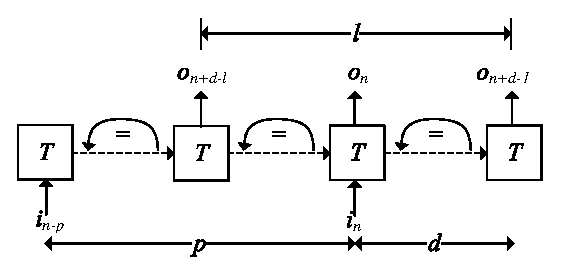
\includegraphics{doubleloop}
% \end{center}
% \caption{The loop-like non-complementary condition}
%   \label{doubleloop}
% \end{figure}

\vspace{0.2cm}
\leftline{\textbf{Unrolling transition relation and checking $PC$}}
\vspace{0.2cm}

\begin{figure}[t]
\begin{center}
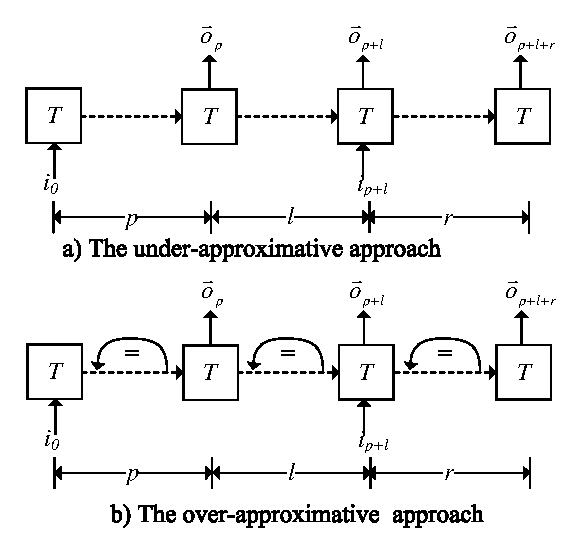
\includegraphics[width=\textwidth]{pcln}
\end{center}
\caption{The $PC$ and $LN$ condition}
  \label{fig_pcln}
\end{figure}

$PC$ is the abbreviation of Parameterized Complementary Condition defined in \cite{ShengYuShen:iccad09},
which is used to determine the existence of the decoder.
Its meaning is intuitively shown in Figure \ref{fig_pcln}a).
$T$ is the encoder's transition relation constructed in previous step,
while $i_n$ and $o_n$ are respectively the input and output letter.
$p$, $d$ and $l$ are respectively the length of the unfolded transition relation,
we also call them the window size.
This figure,
and therefore $PC$,
means that the decoder exists if and only if there exists $p$, $d$ and $l$,
such that the output sequence $<o_{n+d-l},\dots,o_{n+d-1}>$ can uniquely determine the input letter $i_n$.

\vspace{0.2cm}
\leftline{\textbf{Checking $LN$}}
\vspace{0.2cm}

In addition to the $PC$ mentioned in last subsection,
another condition $LN$ is defined in \cite{ShengYuShen:tcad11} to determine the non-existence of the decoder.
Its meaning is intuitively shown in Figure \ref{fig_pcln}b).
It means that the decoder does not exist if and only if there exists $p$, $d$ and $l$,
such that the output sequence $<o_{n+d-l},\dots,o_{n+d-1}>$ can \textbf{NOT} uniquely determine the input letter $i_n$,
and there are three loops on state sequences $<s_{n-p},\dots,s_{n+d-l}>$,$<s_{n+d-l+1},\dots,s_n>$ and $<s_{n+1},\dots,s_{n+d}>$.

If this checking succeeds,
then there does not exist decoder for this encoder and its assertion.
Otherwise,
the window size will be increased and a new iteration will begin.
We have proven in \cite{ShengYuShen:tcad11} that this loop between $LN$ and $PC$ will eventually terminate.

\vspace{0.2cm}
\leftline{\textbf{Characterizing the Boolean function of the decoder}}
\vspace{0.2cm}

If the $PC$ checking succeeds,
then there exists a function that maps the output sequence $<o_{n+d-l},\dots,o_{n+d-1}>$ back to the input letter $i_n$.
This function can be characterized from the Boolean relation shown in Figure \ref{fig_pcln}a),
with the ALLSAT algorithm proposed in \cite{ShengYuShen:tcad}.
Recently,
Liu et al.\cite{Roland:iccad11} proposes a much faster algorithm based on Craig interpolant\cite{Craig} to characterize this function.
The timing and area of the decoder generated by it is comparable to our ALLSAT algorithm.



\section{An Overview of the inferring mode}\label{sec_infer}
The flow of the inferring mode is shown in Figure \ref{fig_infer}.
It is similar to Figure \ref{fig_halting},
with some new steps in gray color.
The assertion is not needed here any more.

\begin{figure}[t]
\centering
\includegraphics[width=\textwidth]{infer}
\caption{The flow of the inferring mode}
\label{fig_infer}
\end{figure}

\vspace{0.2cm}
\leftline{\textbf{Ruling out invalid configuration values}}
\vspace{0.2cm}

If the $LN$ checking succeeds,
an invalid configuration value that leads to the non-existence of the decoder can be obtained from the satisfying assignment returned from the minisat SAT solver\cite{EXTSAT}.
We can simply rule out this invalid configuration value and return to the previous step to check $LN$ again.
But to reduce the runtime overhead,
we propose an algorithm in \cite{ShengYuShen:iccad11} to enlarge this value to a larger set of invalid configuration values with Craig interpolant\cite{Craig},
and rule out them altogether.

The inner loop between this step and the Checking $LN$ step will eventually terminate after such invalid configuration values are all ruled out.
Then the window size is increased to check $PC$ again.

\begin{figure}[b]
\centering
\includegraphics[width=\textwidth]{fdtest_all}
\caption{The two SAT instances that discover decoders and infer precondition formulas}
\label{fig_fdtest}
\end{figure}

We have proven in \cite{ShengYuShen:iccad11} that the outer loop between $LN$ and $PC$ will eventually terminate.
Assume that the set of all configuration values ruled out is $NA$,
then the final inferred assertion is $\wedge_{na\in NA}\neg na$.

\vspace{0.2cm}
\leftline{\textbf{Discovering all decoders' Boolean relations}}
\vspace{0.2cm}

The final inferred assertion is a formula that actually contains many different configuration values.
This means that there may exist multiple decoders for this inferred assertion.

Thus,
our job here is to find out the set of all decoders' Boolean relations $\{R_1,\dots,R_n\}$ step by step.
Assume that we have already discovered a set of decoders' Boolean relations $\{R_1,\dots,R_{m}\}$.
To test whether it contains $\{R_1,\dots,R_n\}$,
that is,
whether all decoders have already been discovered,
we construct the SAT instance shown in Figure \ref{fig_fdtest}a) based on functional dependency\cite{funcdep}.

In Figure \ref{fig_fdtest}a),
we denote $i_n$ as $Y$,
and $<o_{n+d-l},\dots,o_{n+d-1}>$ as $X$,
and the configuration value as $c$.
$R(c,X,Y)$ is the Boolean relation shown in Figure \ref{fig_pcln}a) that succeeds in checking $PC$.

According to \cite{ShengYuShen:tcad12},
if this SAT instance is unsatisfiable,
then all decoders' have been discovered;
Otherwise,
we can discover a new decoder's Boolean relation by assigning the satisfying assignment of $c$ to $R$.

A new round of functional dependency test will be perform again until no more decoder can be discovered.
After that these Boolean relations will be used to characterize their corresponding decoders' Boolean functions.

\vspace{0.2cm}
\leftline{\textbf{Inferring precondition formulas}}
\vspace{0.2cm}

Assume that $\{R_1,\dots,R_{m}\}$ is the set of all decoders' Boolean relations discovered in last step,
and $\{IA_1,\dots,IA_{m}\}$ is their corresponding set of configuration letters.
To help the user determine which $R_i$ in $\{R_1,\dots,R_{m}\}$ is the correct decoder,
we need to characterize each $IA_i$ in $\{IA_1,\dots,IA_{m}\}$.

Assume $Y$ and all $Y_i$ in Figure \ref{fig_fdtest}a) are vectors of the same length $v$,
and the $j$-th bit of them are respectively $Y^{j}$ and $Y_i^{j}$.
If we can characterize the precondition formulas $IA^j_i$ for the $j$-th bit of $IA_i$,
then $IA_i$ can be defined as $\bigwedge _{j=0}^{v-1} IA^j_i$. 

To achieve this goal, 
we construct the unsatisfiable SAT instance shown in Figure \ref{fig_fdtest}b),
which represents a functional dependency problem.
We can characterize $IA^j_i$ with the functional dependency algorithm proposed by Lee et al. \cite{funcdep} with the two formulas $A$ and $B$.
%\begin{figure}[t]
%\centering
%\includegraphics[width=0.75\textwidth]{fdtest_simple}
%\caption{The SAT instance that infers precondition formulas}
%\label{fig_fdtest_simple}
%\end{figure}



\section{Experimental results}\label{sec_exp}
The benchmarks used in experiments include several complex encoders from industrial projects,
a PCI-E\cite{PCIESPEC} physical coding module,
two XGXS and XFI encoders that are compatible to 10G Ethernet\cite{IEEE80232002} standard,
an Ethernet module from Sun's OpenSparc T2 processor,
and a 66-bit scrambler used to ensure that a data sequence has sufficient 0-1 transitions.

According to \cite{ShengYuShen:tcad11},
when given the assertion,
%no matter correct or not,
the synthesis mode can determine the existence of the decoders within 40 seconds,
and builds the decoders within 10 seconds with an algorithm similar to Liu et al.\cite{Roland:iccad11}.
Moreover,
we insert some bugs into these encoders,
which generate the same output letter for two different input letters.
CompSyn successfully detects all these bug within 10 seconds.

According to \cite{ShengYuShen:iccad11,ShengYuShen:tcad12},
when the assertions are not known,
the inferring mode can infer assertions, generate decoders and infer these decoders' precondition formulas in 400 seconds.
Moreover,
only two out of the five benchmarks have two decoders,
while the other three have only one decoder.
This means that,
in most cases,
our algorithm generates only one decoder.
For other cases with multiple decoders,
the user need to inspect $\{IA_1,\dots,IA_{m}\}$ to select the correct decoder.

For example,
for the two decoders of the most complex XFI encoder that compliant to 10G Ethernet standard\cite{IEEE80232002},
their corresponding $IA_1$ is $RESET~\&$ $!TEST\_MODE$,
while $IA_2$ is $!RESET~\&~!TEST\_MODE~\&~DATA\_VALID$.
The essential difference between them is the value of $RESET$.
By inspecting the Verilog source code of XFI,
we find that the $RESET$ is used to reset the XFI encoder when it is $True$.
So the XFI encoder will work in normal mode when $RESET$ is $False$.
So the second decoder is the correct decoder.
The dynamic simulation had also confirmed its correctness.

In this process,
the user only need to inspect the meaning of one configuration pin,
instead of all 120 configuration pins of the XFI encoder.
In this way,
the human effort in specifying assertion and selecting the correct decoder is significantly reduced.

\section{Conclusions}\label{sec_conclude}
The CompSyn tool can inferring correct assertions and generate decoder circuits for several complex encoders.
Furthermore,
it can significantly reduce the human effort in specifying assertion and selecting the correct decoder.


% \section*{Acknowledgment}
% The authors would like to thank the anonymous reviewers for their hard work.

% This work was funded by Projects 60603088 and 61070132 supported by National Natural Science Foundation of China.

\begin{thebibliography}{4}

\bibitem{ShengYuShen:iccad09}
Shen, S.,
Zhang, J.,
Qin, Y.,
Li, S.
:
Synthesizing Complementary Circuits Automatically.
In: ICCAD'09,
pp. 381--388.
IEEE Press,
New York (2009)

\bibitem{ShengYuShen:tcad}
Shen, S.,
Qin, Y.,
Wang, K.,
Xiao, L.,
Zhang, J.,
Li, S.
:
Synthesizing Complementary Circuits Automatically.
IEEE transaction on CAD of Integrated Circuits and Systems
29(8),
1191--1202
(2010)

\bibitem{ShengYuShen:tcad11}
Shen, S.,
Qin, Y.,
Xiao, L.,
Wang, K.,
Zhang, J.,
Li, S.
:
A halting algorithm to determine the existence of the decoder.
IEEE transaction on CAD of Integrated Circuits and Systems
30(10),
1191--1202
(2011).

\bibitem{ShengYuShen:iccad11}
Shen, S.,
Qin, Y.,
Zhang, J.,
Li, S.
:
Inferring Assertion for Complementary Synthesis.
\emph{accepted by ICCAD11}.

\bibitem{ShengYuShen:tcad12}
Shen, S.,
Qin, Y.,
Xiao, L.,
Wang, K.,
Zhang, J.,
Li, S.
:
Inferring Assertion for Complementary Synthesis.
submitted to IEEE transaction on CAD of Integrated Circuits and Systems.

\bibitem{Roland:iccad11}
Liu H.,
Chou Y.C.,
Lin C.H.,
Jiang J.-H.~R.
:
Completely Automatic Decoder Synthesis.
\emph{accepted by ICCAD11}.


% \bibitem{Cofact}
% Ganai, M.K.,
% Gupta, A.,
% Ashar, P.
% :
% Efficient SAT-based unbounded symbolic model checking using circuit cofactoring.
% In: 2004 International Conference on Computer-Aided Design,
% pp. 510--517.
% IEEE Press,
% New York (2004)


\bibitem{Craig}
Craig, W.
:
Linear reasoning: A new form of the Herbrand-Gentzen theorem.
J. Symbolic Logic. 22(3), 250--268 (1957)


\bibitem{EXTSAT}
E\'en, N.,
S\"orensson, N.
:
Extensible SAT-solver.
In: Giunchiglia, E., Tacchella, A. (eds.)
SAT 2003.
LNCS, vol. 2919,
pp. 502--518.
Springer, Heidelberg (2003)

\bibitem{PCIESPEC}
PCI Express Base Specification Revision 1.0.
\url{http://www.pcisig.com}

\bibitem{IEEE80232002}
\emph{IEEE Standard for Information technology Telecommunications and
  information exchange between systems Local and metropolitan area networks
  Specific requirements Part 3: Carrier Sense Multiple Access with Collision
  Detection (CSMA/CD) Access Method and Physical Layer Specifications
  Amendment: Media Access Control (MAC) Parameters, Physical Layers, and
  Management Parameters for 10 Gb/s Operation}, IEEE Std. 802.3, 2002.

\bibitem{funcdep}
Lee C.-C. ,
Jiang J.-H.~R. ,
Huang C.-Y. ,
Mishchenko A.
:
Scalable exploration of functional dependency by interpolation and incremental SAT solving.
In: ICCAD'07,
pp. 227--233.
IEEE Press,
New York (2007)


% \bibitem{CHAFF}
% Moskewicz, M.,
% Madigan, C.,
% Zhao, Y.,
% Zhang, L.,
% Malik, S.
% :
% Chaff: Engineering an Efficient SAT Solver.
% In: 38th Design Automation Conference,
% pp. 530--535.
% IEEE Press,
% New York (2001)



% \bibitem{grasp}
% Silva, J.,
% Sakallah, K.
% :
% GRASP - a new search algorithm for satisfiability.
% In: 1996 International Conference on Computer-Aided Design,
% pp. 220--227.
% IEEE Press,
% New York (1996)


% \bibitem{BERKMIN}
% Goldberg, E.,
% Novikov, Y.
% :
% BerkMin: A Fast and Robust Sat-Solver.
% In: 2002 Design, Automation and Test in Europe Conference and Exposition,
% pp. 142--149.
% IEEE Press,
% New York (2002)


% \bibitem{interp_Krajicek} Krajicek, J.: Interpolation theorems, lower bounds for proof systems,
% and independence results for bounded arithmetic.
% J. Symbolic Logic 62(2), 457--486 (1997)


% \bibitem{interp_Pudlak} Pudlak, P.: Lower bounds for resolution and cutting plane proofs and
% monotone computations.
% J. Symbolic Logic 62(3), 981--998 (1997)


% \bibitem{interp_McMillan}
% McMillan, K.L.
% :
% Interpolation and SAT-based model checking.
% In: Hunt, W.A., Somenzi, F. (eds.)
% CAV 2003.
% LNCS, vol. 2725,
% pp. 1--13.
% Springer, Heidelberg (2003)

% \bibitem{MEALY} Mealy, G.H.: A method for synthesizing sequential circuits.
% Bell Systems Technical Journal 34(5), 1045--1079 (1955)

% \bibitem{RecDiam}
% Kroening, D.,
% Strichman, O.
% :
% Efficient Computation of Recurrence Diameters.
% In: Zuck, L.D., Attie, P.C., Cortesi, A., Mukhopadhyay, S. (eds.)
% VMCAI 2003.
% LNCS, vol. 2575,
% pp. 298--309.
% Springer, Heidelberg (2003)

% \bibitem{ShengYuShen:fmcad10}
% Shen, S.,
% Qin, Y.,
% Zhang, J.,
% Li, S.
% :
% A Halting Algorithm to Determine the Existence of Decoder.
% In: 10th International Conference on Formal Methods in Computer-Aided Design,
% pp. 91--100.
% IEEE Press,
% New York (2010)

% \bibitem{dim_syn}
% Gulwani, S.
% :
% Dimensions in program synthesis.
% In: 12th International ACM SIGPLAN Conference on Principles and Practice of Declarative Programming,
% pp. 13--24.
% ACM Press,
% New York (2010)
%
% \bibitem{prog_inv}
% Edsger W. Dijkstra.
% Program Inversion.
% in Program Construction,
% pp 54-57,
% 1978.
%
%
% \bibitem{mtd_autoProginv}
% Gl\"{u}ck, R.,
% Kawabe, M.
% :
% A method for automatic program inversion based on LR(0) parsing.
% Fundam. Inf. 66(4), 367--395 (2005)
%
% \bibitem{prog_inv_rev}
% Srivastava, S.,
% Gulwani, S.,
% Chaudhuri, S.,
% Foster, J.
% :
% Program inversion revisited.
% Technical Report MSR-TR-2010-34, Microsoft Research (2010)
%
%
%
% \bibitem{converter_date08}
% Avnit, K.,
% D'Silva, V.,
% Sowmya, A.,
% Ramesh, S.,
% Parameswaran, S.
% :
% A Formal Approach To The Protocol Converter Problem.
% In: 2008 Design, Automation and Test in Europe Conference and Exposition,
% pp. 294--299.
% IEEE Press,
% New York (2008)
%
%
% \bibitem{converter_date09}
% Avnit, K.,
% Sowmya, A.
% :
% A formal approach to design space exploration of protocol converters.
% In: 2009 Design, Automation and Test in Europe Conference and Exposition,
% pp. 129--134.
% IEEE Press,
% New York (2009)


% \bibitem{converter_tacas10}
% Avnit, K.,
% Sowmya, A.,
% Peddersen, J.
% :
% ACS: Automatic Converter Synthesis for SoC Bus Protocols.
% In: Esparza, J., Majumdar,R. (eds.)
% TACAS 2010.
% LNCS, vol. 6015,
% pp. 343--348.
% Springer, Heidelberg (2010)

\end{thebibliography}



\end{document}
